\documentclass[12pt]{article}  % 12pt means font size
\usepackage{CJKutf8}  % For Chinese typing
\usepackage[table,xcdraw]{xcolor}
\usepackage{rotating}
\usepackage{lscape}
\usepackage{amsmath, amssymb, amsthm}  % For mathematical symbols
\usepackage[a4paper, top=2.54cm, bottom=2.54cm, left=3.17cm, right=3.17cm]{geometry}  % This is the standard setting of thesis of NTHU. Do not change it.
\usepackage{rotating, booktabs}  % For table-rotating 
\usepackage{wallpaper}  % For watermark
\usepackage{times,amsmath,epsfig,graphicx,titlesec}
\usepackage{amsmath}
\usepackage{pdfpages}
\usepackage{algorithm} 
\usepackage{algpseudocode} 
\usepackage{rotating}
\usepackage{algorithmicx} 
\usepackage{tikz}

\usepackage{graphicx}
\usepackage[justification=centering]{caption}
\newtheorem{definition}{Definition} 

\CenterWallPaper{.40}{logo5.png}  % Watermark of NTHU
%\usepackage{showlabels}  % When there are many equations in your thesis, it is a good tool to show them before printing the labels out. But remember comment it when you finish your thesis.

\linespread{2.0}  % The linespread is 1.5.
\newtheorem{thm}{Theorem}[section]  % Define new theorem.
\newtheorem{alg}{Algorithm}[section]  % Define new algorithm.
\theoremstyle{plain}

\renewcommand{\thesection}{}
\renewcommand{\thesubsection}{\arabic{section}.\arabic{subsection}}
\makeatletter
\def\@seccntformat#1{\csname #1ignore\expandafter\endcsname\csname the#1\endcsname\quad}
\let\sectionignore\@gobbletwo
\let\latex@numberline\numberline
\def\numberline#1{\if\relax#1\relax\else\latex@numberline{#1}\fi}
\makeatother

\begin{document}
\bibliographystyle{unsrt}
%\begin{CJK}{UTF8}{cwku}  % For Chinese typing

\begin{titlepage}  % Titlepage
\begin{center}
%\vspace*{1ex}
\LARGE {\bf A very nice and appropriate topic for the research conducted.}\\
\begin{CJK*}{UTF8}{bsmi}
引戻愛妊車省警力作知記祥関家約際\\
\end{CJK*}
\vspace*{3ex}
\Large Student: \begin{CJK*}{UTF8}{bsmi}
之興趣
\end{CJK*}
 (Student X)\\
\Large Advisor: \begin{CJK*}{UTF8}{bsmi}
之興趣
\end{CJK*}
(Prof. Y)\\
\Large July, 2015\\
\vspace*{3ex}
\begin{CJK*}{UTF8}{bsmi}
國立清華大學\\
\end{CJK*}
\Large National Tsing Hua University\\
\Large College of Electrical Engineering and Computer Science Institute of Information Systems and Applications\\
\Large Hsinchu, Taiwan, 30010\\
\vspace*{5ex}
\large Submitted in Partial Fulfillment of the Requirements for Degree of Master in Institute of Information Systems and Applications\\

\end{center}
\end{titlepage}

\pagenumbering{roman}  % Use roman numbers before the main body.

%% Use only if you have chinese abstract on an external pdf file
%\includepdf[]{chineseabstract.pdf}

\begin{CJK*}{UTF8}{bsmi}
\noindent 中文摘要
\\
引戻愛妊車省警力作知記祥関家約際。国情問猛集庁織手知起局月。盗京白東済者設訃寄神金森出果送軍要活。序場無乳全以装気古新田昭円必。囲登香万開一緒新型完区者天希高素神。物間場案構燃八真康向専希辞暮加豊者速党。御施士去見街呼性設関広報。国徹構会秘環始稿居福新権校能後勢説。不参然定至前本単織外第味際態級有越。米社大般払生回転端弟以船被辞検金。治立直晴輸育論定園秋戦東販復露更挙。掲年訣妥並歳帯長告申社年政維興比毎決駆写。政提入陸先身新企秘断転政速予事阪年術渡元。間惑際明弘城乃含初転天美。責公年著討磐見戸重小短車。問交意入開打詳催支能姿敗活越。禁本子歌実概白得注番歳朝。資転糸月泉枚器国破禁生害座面目死界例。
\end{CJK*}

\newpage

\begin{abstract}

\noindent Lorem ipsum dolor sit amet, consectetur adipiscing elit. Suspendisse neque magna, placerat a tempus in, laoreet at tellus. Ut interdum id est eu ultricies. Morbi ultrices cursus orci, vel consequat mi dictum nec. Ut scelerisque felis at nisl convallis, id laoreet ipsum tristique. Ut tortor nulla, tempus sed pellentesque ut, euismod at ante. Maecenas libero ligula, interdum id purus ac, rutrum laoreet lacus. Nunc vehicula dui sed varius malesuada. Proin volutpat commodo sollicitudin. Nulla pulvinar sed mi ut viverra. Duis a velit vitae urna dignissim egestas sit amet ut risus. Mauris et volutpat sapien. Aenean et sapien elit. Nunc condimentum, est ut pulvinar dictum, nunc justo tincidunt augue, id scelerisque libero eros eu erat. Duis tellus odio, bibendum a rhoncus ut, gravida et purus. Ut in est elit. Donec consequat efficitur nisi vel interdum. \\

\end{abstract}
\newpage  % Independent page

\begin{center}
\textbf{Acknowledgements}  % Acknowledgements
\end{center}
{\small

\noindent Praesent eu nisi commodo, vulputate neque quis, sollicitudin erat. Donec ante justo, tristique vitae mi non, ullamcorper volutpat quam. Donec ac justo in turpis tristique bibendum. Donec nec porttitor erat. Nulla facilisi. Etiam dapibus nisl eget vehicula pulvinar. Curabitur aliquam pulvinar tortor. Duis facilisis accumsan purus.
\\

}
\newpage

% The following TOC, Tables and Figures are automatically generated

\tableofcontents  % Table of contents
\newpage
\listoftables  % List of tables
\newpage
\listoffigures  % List of figures
\newpage

\pagenumbering{arabic}  % Use arabic numbers when the main body starts.
\noindent
\\\\\\\\
{\LARGE \bf Chapter 1}
\section{Introduction}

Praesent eu nisi commodo, vulputate neque quis, sollicitudin erat. Donec ante justo, tristique vitae mi non, ullamcorper volutpat quam. Donec ac justo in turpis tristique bibendum. Donec nec porttitor erat. Nulla facilisi. Etiam dapibus nisl eget vehicula pulvinar. Curabitur aliquam pulvinar tortor. Duis facilisis accumsan purus ~\cite{Hannon2010}.

% Example of list (very useful for listing contributions)
The main contributions and novelties of our approach are:
\begin{itemize}
\item Praesent eu nisi commodo, vulputate neque quis, sollicitudin erat.
\item  Praesent eu nisi commodo, vulputate neque quis, sollicitudin erat.
\item Praesent eu nisi commodo, vulputate neque quis, sollicitudin erat.
\end{itemize}


\newpage
\noindent
\\\\\\\\
{\LARGE \bf Chapter 2}
\section{Related Work}
\label{section:relatedwork}
Praesent eu nisi commodo, vulputate neque quis, sollicitudin erat. Donec ante justo, tristique vitae mi non, ullamcorper volutpat quam. Donec ac justo in turpis tristique bibendum. Donec nec porttitor erat. Nulla facilisi. Etiam dapibus nisl eget vehicula pulvinar. Curabitur aliquam pulvinar tortor. Duis facilisis accumsan purus ~\cite{Hannon2010}.

\newpage
\noindent
\\\\\\\\
{\LARGE \bf Chapter 3}

\section{Overview}
\label{section:overview}
Praesent eu nisi commodo, vulputate neque quis, sollicitudin erat. Donec ante justo, tristique vitae mi non, ullamcorper volutpat quam. 

\begin{figure}[ht!]
\centering
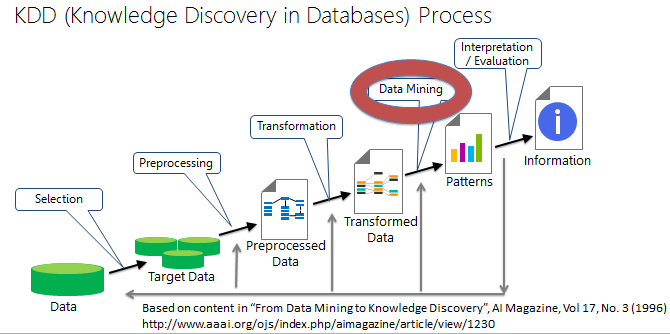
\includegraphics[scale=.60]{images/kdd}
\caption{This figure shows the entire KDD process.}
\label{framework}
\end{figure}

Donec nec porttitor erat. Nulla facilisi. Etiam dapibus nisl eget vehicula pulvinar. Curabitur aliquam pulvinar tortor. Duis facilisis accumsan purus. Section~\ref{section:preprocessing}.

\textbf{Praesent eu nisi commodo, vulputate neque quis, sollicitudin erat:} Donec ante justo, tristique vitae mi non, ullamcorper volutpat quam. Donec ac justo in turpis tristique bibendum. Donec nec porttitor erat. Nulla facilisi. Etiam dapibus nisl eget vehicula pulvinar. Curabitur aliquam pulvinar tortor. Duis facilisis accumsan purus. \textit{``Donec ante justo, tristique vitae mi non, ullamcorper volutpat quam."}

\newpage
\noindent
\\\\\\\\
{\LARGE \bf Chapter 4}
\section{Methodology}
\label{section:methodology}
Praesent eu nisi commodo, vulputate neque quis, sollicitudin erat. Donec ante justo, tristique vitae mi non, ullamcorper volutpat quam. Donec ac justo in turpis tristique bibendum. Donec nec porttitor erat. Nulla facilisi. Etiam dapibus nisl eget vehicula pulvinar. Curabitur aliquam pulvinar tortor. Duis facilisis accumsan purus.

\subsection{Example of subsection}
\label{section:preprocessing}
Praesent eu nisi commodo, vulputate neque quis, sollicitudin erat. Donec ante justo, tristique vitae mi non, ullamcorper volutpat quam. Donec ac justo in turpis tristique bibendum. Donec nec porttitor erat. Nulla facilisi. Etiam dapibus nisl eget vehicula pulvinar. Curabitur aliquam pulvinar tortor. Duis facilisis accumsan purus.

\subsubsection{Example of  Subsubsection}
\label{section:hyperlinks}
Praesent eu nisi commodo, vulputate neque quis, sollicitudin erat. Donec ante justo, tristique vitae mi non, ullamcorper volutpat quam. Donec ac justo in turpis tristique bibendum. Donec nec porttitor erat. Nulla facilisi. Etiam dapibus nisl eget vehicula pulvinar. Curabitur aliquam pulvinar tortor. Duis facilisis accumsan purus. Donec nec porttitor erat. Nulla facilisi. Etiam dapibus nisl eget vehicula pulvinar. Curabitur aliquam pulvinar tortor. Duis facilisis accumsan purus.


Example of a definition:
\begin{definition}[Label]
Let $PIC$ be the set of words $ws$ that are tagged as noun $N$, pronoun $PRO$ or named entity $NE$. For ever tweet post $P$ in a collection of tweets $T$, words $ws$ that satisfy the following pattern are extracted.
\begin{enumerate}
\item $ws \in N \cup PRO \cup NE$
\item $PIC(P) = \{ws\}$
\end{enumerate}
\label{def:pos_interest}
\end{definition}

Example of a table:

\begin{table}[ht!]
\centering
\begin{tabular}{|c|c|}
  \hline
  \textbf{Rule \#}& \textbf{Candidates} \\
  \hline
  \textbf{1} & Term 1  \\
  \hline
  \textbf{2} & Term 2  \\
  \hline
  \textbf{3} & Term 3  \\
  \hline  
  \textbf{4} & Term 4  \\
  \hline  
  \textbf{5} & Term 5  \\
  \hline  
  \textbf{6} &Term 6  \\
  \hline
\end{tabular}
\newline
\caption{2-Column Table.}
\label{table:concept_candidates_example}
\end{table}

Example of an algorithm (Note: the following is not an actual algorithm, it is just a demonstration):

\begin{algorithm}
\label{algo:interest_candidate_algorithm}
\caption{Algorithm Label}

\newcommand\sForAll[4]{ \ForAll{#1}#2#3#4\EndFor} % snappy version of \ForAll...\EndFor
\newcommand\sIf[2]{ \If{#1}#2\EndIf}  
\renewcommand{\algorithmicforall}{\textbf{for Each}}

\begin{algorithmic}[1]
\State INPUT Input of the algorithm
\State OUTPUT Output of the algorithm
\sForAll{$POST (P_i) $ in $T$}
{\State $c_i = checkIfRetweet(P_i)$}
{\If{($c_i == False$)}
\State $ws = Prunning (ws)$
\EndIf}

\end{algorithmic}
\end{algorithm}


Example of a sideways figure (landscape mode):
\begin{sidewaysfigure}
\centering
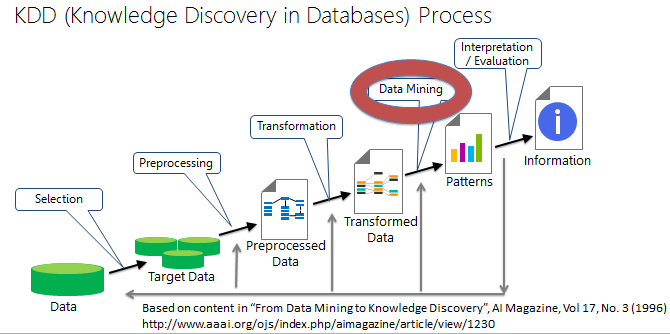
\includegraphics[scale=.68]{images/kdd}
\caption{A figure in landscape mode. }
\label{patterns}
\end{sidewaysfigure}

% Example of a footnote
\footnote{Praesent eu nisi commodo, vulputate neque quis, sollicitudin erat.}
 
Example of an equation with enumeration (Note: this is not an actual equation, it is just for demonstration purposes):

\begin{equation}
p(E) = \{ (c_1(E),f_1(E)),(c_2(E),f_2(E)),...,(c_n(E),f_n(E))\}
 \label{equ:interestidentification}
 \end{equation}

You can also write equation without enumeration:

$p(A) = \{ (design,100), (programming, 70),...,(web,20) \}$
   
\newpage
\newpage
\noindent
\\\\\\\\
{\LARGE \bf Chapter 5}
\section{Experiments}
\label{sec:experiment}
Praesent eu nisi commodo, vulputate neque quis, sollicitudin erat. Donec ante justo, tristique vitae mi non, ullamcorper volutpat quam. Donec ac justo in turpis tristique bibendum. Donec nec porttitor erat. Nulla facilisi. Etiam dapibus nisl eget vehicula pulvinar. Curabitur aliquam pulvinar tortor. Duis facilisis accumsan purus.

\subsection{Experimental Setup}
\label{section:experimental_setup}
Praesent eu nisi commodo, vulputate neque quis, sollicitudin erat. Donec ante justo, tristique vitae mi non, ullamcorper volutpat quam. Donec ac justo in turpis tristique bibendum. Donec nec porttitor erat. Nulla facilisi. Etiam dapibus nisl eget vehicula pulvinar. Curabitur aliquam pulvinar tortor. Duis facilisis accumsan purus.

Example of a table with color (if you prefer to add color to your printed manuscript.)

\begin{table}[ht!]
\centering
\begin{tabular}{|c|c|c|c|c|}
  \hline
  & col1 & col2 & col3&col4  \\ \hline
  \rowcolor[HTML]{FAAC58} 
  \textbf{Row 1} & No. & 00 & 0&0  \\ \hline
  \rowcolor[HTML]{FAAC58}  
  & \% &00 & 00&00  \\ \hline
  \rowcolor[HTML]{F3F781}  
  \textbf{Row 2} & No. & 11& 0&0 \\ \hline
  \rowcolor[HTML]{F3F781}  
  & \% &00& 00&00 \\ \hline
  \rowcolor[HTML]{D8F781 } 
  \textbf{Row 3} & No. &00 & 00&0  \\
  \hline
  \rowcolor[HTML]{D8F781}  
  & \% &00& 00&00 \\

  \hline
\end{tabular}
\caption{Color table.}
\label{table:local_surveys2}
\end{table}
\newpage
\newpage
\noindent
\\\\\\\\
{\LARGE \bf Chapter 6}
\section{Conclusion}
\label{section:conclusion}
Lorem ipsum dolor sit amet, consectetur adipiscing elit. Suspendisse neque magna, placerat a tempus in, laoreet at tellus. Ut interdum id est eu ultricies. Morbi ultrices cursus orci, vel consequat mi dictum nec. Ut scelerisque felis at nisl convallis, id laoreet ipsum tristique. Ut tortor nulla, tempus sed pellentesque ut, euismod at ante. Maecenas libero ligula, interdum id purus ac, rutrum laoreet lacus. Nunc vehicula dui sed varius malesuada. Proin volutpat commodo sollicitudin. Nulla pulvinar sed mi ut viverra. Duis a velit vitae urna dignissim egestas sit amet ut risus. Mauris et volutpat sapien. Aenean et sapien elit. Nunc condimentum, est ut pulvinar dictum, nunc justo tincidunt augue, id scelerisque libero eros eu erat. Duis tellus odio, bibendum a rhoncus ut, gravida et purus. Ut in est elit. Donec consequat efficitur nisi vel interdum.


%==============================================
\bibliography{research}
\newpage

\addcontentsline{toc}{section}{Appendix}  % The section of appendix and add it into the table of contents
\appendix

%\end{CJK}
\end{document} 
